\chapter[SCP-152 末日之书]{
    SCP-152 Book of Endings\\
    SCP-152 末日之书
}

\label{chap:SCP-152}

\begin{figure}[H]
    \centering
    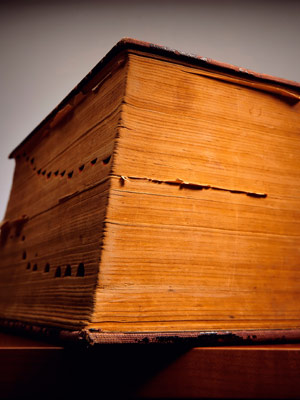
\includegraphics[width=0.5\linewidth]{images/SCP-152.jpg}
    \caption*{SCP-152侧面图}
\end{figure}

\bb{项目编号:}SCP-152

\bb{项目等级:}Safe

\bb{特殊收容措施:}SCP-152放置在49区一个封闭的舱室里,并自此被称为“阅览室”。等级2以下人员无权进入阅览室。阅览室配备了一盏吊灯,一台监视器,一台装好了打印纸和墨水的扫描-复印-打印机,一把标准办公椅,还有一张标准办公桌来摆放SCP-152.当不使用时,SCP-152应翻到最后一页,这样可以马上看见有任何更新。一个守卫将布置在外面防止未授权人员进入阅览室。所有人员都被指示在靠近阅览室时保持安静。

\bb{描述:}SCP-152是一本巨大的,精装的,有金属边角的书本。黑墨水的字符写在似乎是上等牛皮纸的纸张上。数个目录上的内容,都是描述天启级的灾难事件,虽然不是全部都是XK级世界毁灭剧本,但是一样都是以人类毁灭为结局。这些故事以事件顺序排列,从公元前6000年的太阳异常活动开始,到接近当期日期的数个故事结束。大部分故事都是描写很多末日灾难都是源于基金会现在或者曾经保管过的物品,或者是因为一次超自然现象。当然也记录了很多“传统”的形式,比如核战争或者致命病毒导致的人类灭绝。每个故事描述了灾难发生的细节的前提,直到如何导致地球上的人类灭绝。

可以证实的是SCP-152的文字会自动翻译成读者最熟悉的语言,文字和句式会变成对每个读者来说都意味深长的句式,甚至还会使用一些只有读者明白的俗语;唯一不变的只有其主要思想(就是人类毁灭)。如果有几个人同时观看SCP-152,那么它将切换成第一个对进行阅读的人最熟悉的语言。如果没有人观看目标,目标文字将停留在最后一个读者所熟悉的语言上。偶尔,书上的文字也会以横排显示出没有“翻译”的未知语种。

对于熟知基金会历史的人来说,SCP-152所显示的大部分信息都是准确的,仅仅在末日发生与否上有分歧。 绝大部分情况下,在SCP-152所显示版本的历史中,区别在于一些关键的抉择上的不同,而这(些不同)最终导致了人类的灭绝。

SCP-152几乎抵抗任何改变或者书写的企图。墨水,石墨,木炭以及其他书写材料似乎无法附着在书页上,而且很容易抹去。镭射或者其他热源也无法点燃书页;书页和书页之间只有5微米的间隔,任何外来材料都难以插入。以此看来,SCP-152是不会腐烂的,同时也是难以测定其确切存在时间。

SCP-152会自动更新,新的用黑墨水写好的书页和人类灭亡的故事总是不定期更新,出现在书的最末页;新的故事同样都是描述人类如何灭绝的。当页面空间“写”满后,额外的一张将会出现在末页后,同时SCP-152的书脊也会扩大。当SCP-152被基金会保管后进行了 ███ 次更新。在过去的几次事件中,SCP-152被证实会更新出当前灾难的发生地点。由于最近的记录一直频繁地提到对于基金会有兴趣的存在与组织,包括基金会自己,SCP-152被定期检查是否有任何重要信息。

\bb{附录1:}\ii{这些书上的内容如果被散布到公众去对我们来说是很危险的,有什么理由真的需要研究它么?过时的灾难假设剧本不是我们要关心的,我们现在有一大堆真正的麻烦要关心。}-05-█

\bb{附录2:}\ii{这本书上关于多灾多难的地球的准确描述对于当前的业务拥有很好的指导作用。另外,它也对一些我们所持有的SCP项目一旦失控产生的后果给了一个清晰的远景。我认为所有有权限的研究人员都应该抽空来读一读最后50页,这会让他们深刻的理解一下他们的工作是多么重要。“只因少了一个钉子”和诸如此类的。}-Jansen博士

\bb{附录3:}\ii{Jansen,最后50页书上的一半都是写得基金会如何搞砸和害死所有人的。}-05-█

\bb{附录4:}\ii{就像我说的,它提供了一点点远景。}-Jansen博士

\bb{事故报告:152-05:}在████年█月██日的晚上,负责监视器的守卫注意到SCP-152从阅览室消失了。无论如何,在她通过交换机报告之后,SCP-152又重新出现了,而且末页又更新了一张。因为这已经是第5次书本忽然消失和出现(参考事故报告152-01到152-04),于是用一台高速摄像机,装在SCP-152放置的那个桌子里的一台高灵敏电子秤,以及一个会在电子秤数值变化后启动的警报装置进行了一个简单实验。在之后的三次“更新”中SCP-152都没有触发警报,而高速摄像机显示SCP-152每次都是在1秒内消失掉。

\bb{附录5:}\ii{我假设这本书不是这么“更新”的……它应该是被换了一本,而每次它改变都是我们收到了一个它的新版本。我对它从哪来很有兴趣。}-Jansen博士
